\documentclass[11pt]{beamer}
% \usetheme{Boadilla}
  \usetheme{default}


% acronyms for text or math mode
\newcommand {\ccast} {\mbox{\small CCAST}}
\newcommand {\cris} {\mbox{\small CrIS}}

\newcommand {\airs} {\mbox{\small AIRS}}
\newcommand {\iasi} {\mbox{\small IASI}}
\newcommand {\idps} {\mbox{\small IDPS}}
\newcommand {\nasa} {\mbox{\small NASA}}
\newcommand {\noaa} {\mbox{\small NOAA}}
\newcommand {\nstar} {\mbox{\small STAR}}
\newcommand {\umbc} {\mbox{\small UMBC}}
\newcommand {\uw}   {\mbox{\small UW}}

\newcommand {\fft}  {\mbox{\small FFT}}
\newcommand {\ifft} {\mbox{\small IFFT}}
\newcommand {\fir}  {\mbox{\small FIR}}
\newcommand {\fov}  {\mbox{\small FOV}}
\newcommand {\for}  {\mbox{\small FOR}}
\newcommand {\ict}  {\mbox{\small ICT}}
\newcommand {\ils}  {\mbox{\small ILS}}
\newcommand {\igm}  {\mbox{\small IGM}}
\newcommand {\opd}  {\mbox{\small OPD}}
\newcommand {\rms}  {\mbox{\small RMS}}
\newcommand {\zpd}  {\mbox{\small ZPD}}
\newcommand {\ppm}  {\mbox{\small PPM}}
\newcommand {\srf}  {\mbox{\small SRF}}
\newcommand {\sdr}  {\mbox{\small SDR}}

\newcommand {\ES} {\mbox{\small ES}}
\newcommand {\SP} {\mbox{\small SP}}
\newcommand {\IT} {\mbox{\small IT}}
\newcommand {\SA} {\mbox{\small SA}}

\newcommand {\ET} {\mbox{\small ET}}
\newcommand {\FT} {\mbox{\small FT}}

% abbreviations, mainly for math mode
\newcommand {\real} {\mbox{real}}
\newcommand {\imag} {\mbox{imag}}
\newcommand {\atan} {\mbox{atan}}
\newcommand {\obs}  {\mbox{obs}}
\newcommand {\calc} {\mbox{calc}}
\newcommand {\sinc} {\mbox{sinc}}
\newcommand {\psinc} {\mbox{psinc}}
\newcommand {\std} {\mbox{std}}

% symbols, for math mode only
\newcommand {\wnum} {\mbox{cm$^{-1}$}}
\newcommand {\lmax} {L_{\mbox{\tiny max}}}
\newcommand {\vmax} {V_{\mbox{\tiny max}}}

\newcommand {\tauobs} {\tau_{\mbox{\tiny obs}}}
\newcommand {\taucal} {\tau_{\mbox{\tiny calc}}}
\newcommand {\Vdc}  {V_{\mbox{\tiny DC}}}

\newcommand {\rIT} {r_{\mbox{\tiny\textsc{ict}}}}
\newcommand {\rES} {r_{\mbox{\tiny\textsc{es}}}}
\newcommand {\robs} {r_{\mbox{\tiny obs}}}

\newcommand {\rITobs} {r_{\mbox{\tiny\textsc{ict}}}^{\mbox{\tiny obs}}}
\newcommand {\rITcal} {r_{\mbox{\tiny\textsc{ict}}}^{\mbox{\tiny cal}}}

\newcommand {\ITmean} {\langle\mbox{\small IT}\rangle}
\newcommand {\SPmean} {\langle\mbox{\small SP}\rangle}


\title{CrIS FOV 5 Anomaly and the \\
       Nonlinearity Correction \\
  \vspace{4mm}
  {****} DRAFT {****} \\
}
\author{H.~E.~Motteler, L.~L.~Strow}
\institute{
  UMBC Atmospheric Spectroscopy Lab \\
  Joint Center for Earth Systems Technology \\
}
\date{\today}
\begin{document}

%----------- slide --------------------------------------------------%
\begin{frame}[plain]
\titlepage
\end{frame}
%----------- slide --------------------------------------------------%
\begin{frame}
\frametitle{introduction}

\begin{itemize}

  \item Bob Knuteson (most recently) and others have shown FOV5 at
    668.125 \wn can have an anomalously warm brightness temperature
    relative to the other FOVs when the 900 \wn window channel is
    cold

  \item we show a corresponding anomaly from the DC level integral
    of the nonlinearity correction, and for that correction, which
    may explain the brightness temp anomaly

\end{itemize}

\end{frame}
%----------- slide --------------------------------------------------%
\begin{frame}
\frametitle{methods}

\begin{itemize}

  \item the nonlinearity correction applied to FOV 5 is
    significantly less than the corrections applied to other FOVs

  \item however the correction applied to FOV 5 relative to the
    other FOVs is slightly greater for spectra with a cold vs a warm
    window region

  \item this is becauce the DC level integral for FOV 5 relative to
    the other FOVs is slightly greater for spectra with a cold vs a
    warm window region

\end{itemize}

\end{frame}
%----------- slide --------------------------------------------------%
\begin{frame}
\frametitle{methods}

\begin{itemize}

  \item we find homogeneous scenes for two cases: warm and cold at
    900 \wn, as follows

  \item LW brightness temperature spectra were compared for all FOVs
    for FOR 15 and 16 from 1--3 Jan 2016.  If the max RMS difference
    between any pair of FOVs was less than 1K and the mean over all
    FOVs at 900 cm-1 was less than 230K, the FOR was saved as a
    ``cold FOR''

  \item similarly, if the max RMS difference between any pair of
    FOVs was less than 1K and the mean over all FOVs at 900 cm-1 was
    greater than 270K, the FOR was saved as a ``warm FOR''.

\end{itemize}

\end{frame}
%----------- slide --------------------------------------------------%
\begin{frame}
\frametitle{methods}

\begin{itemize}

  \item we found hundreds of warm FORs but only 7 cold FORs over the
    3-day period.  The cold FORs were then further ordered by their
    temperature at 668.125 \wn, and we took the warmest three (at
    243, 242, and 241K) and paired these with warm sets with similar
    temperatures at 668.125 \wn

\end{itemize}

\end{frame}
%----------- slide --------------------------------------------------%
\begin{frame}
\frametitle{test set 1}
\begin{center}
  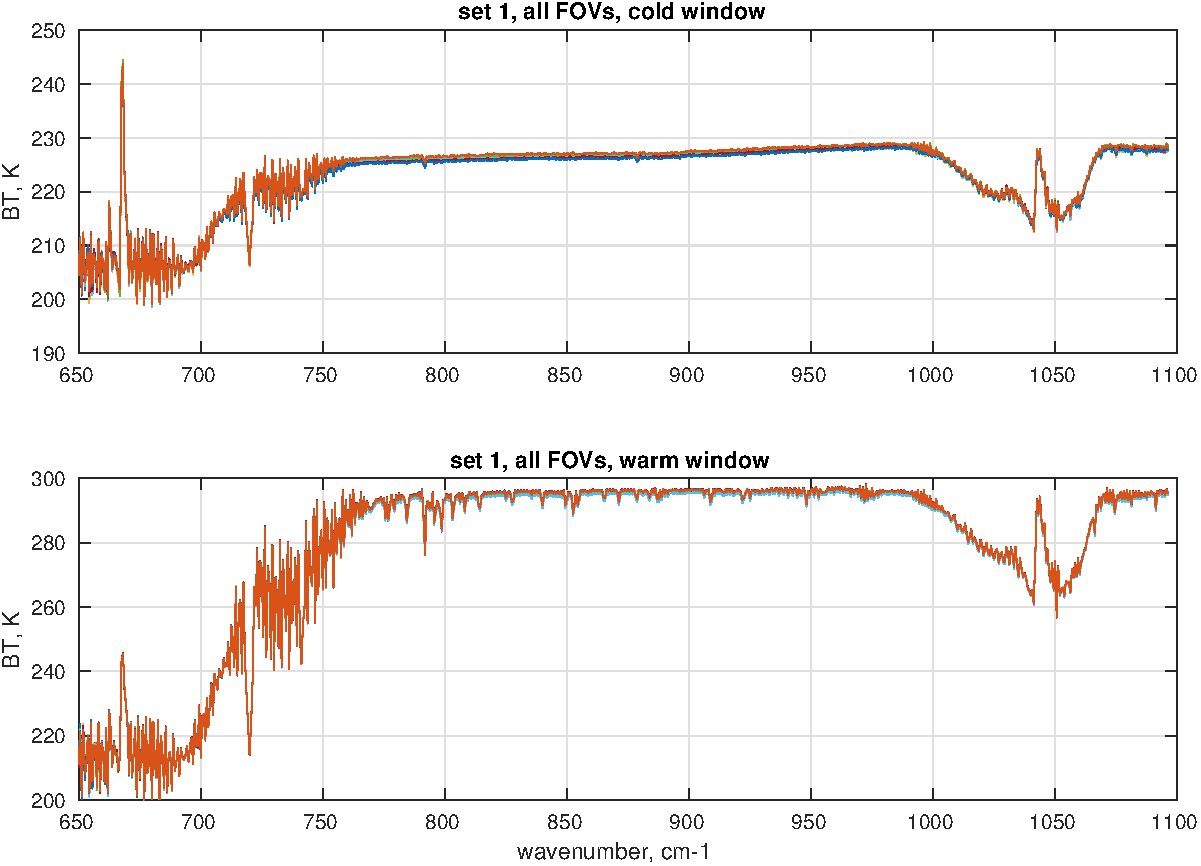
\includegraphics[scale=0.5]{figures/set1_all.pdf}
\end{center}
\end{frame}
%----------- slide --------------------------------------------------%
\begin{frame}
\frametitle{test set 2}
\begin{center}
  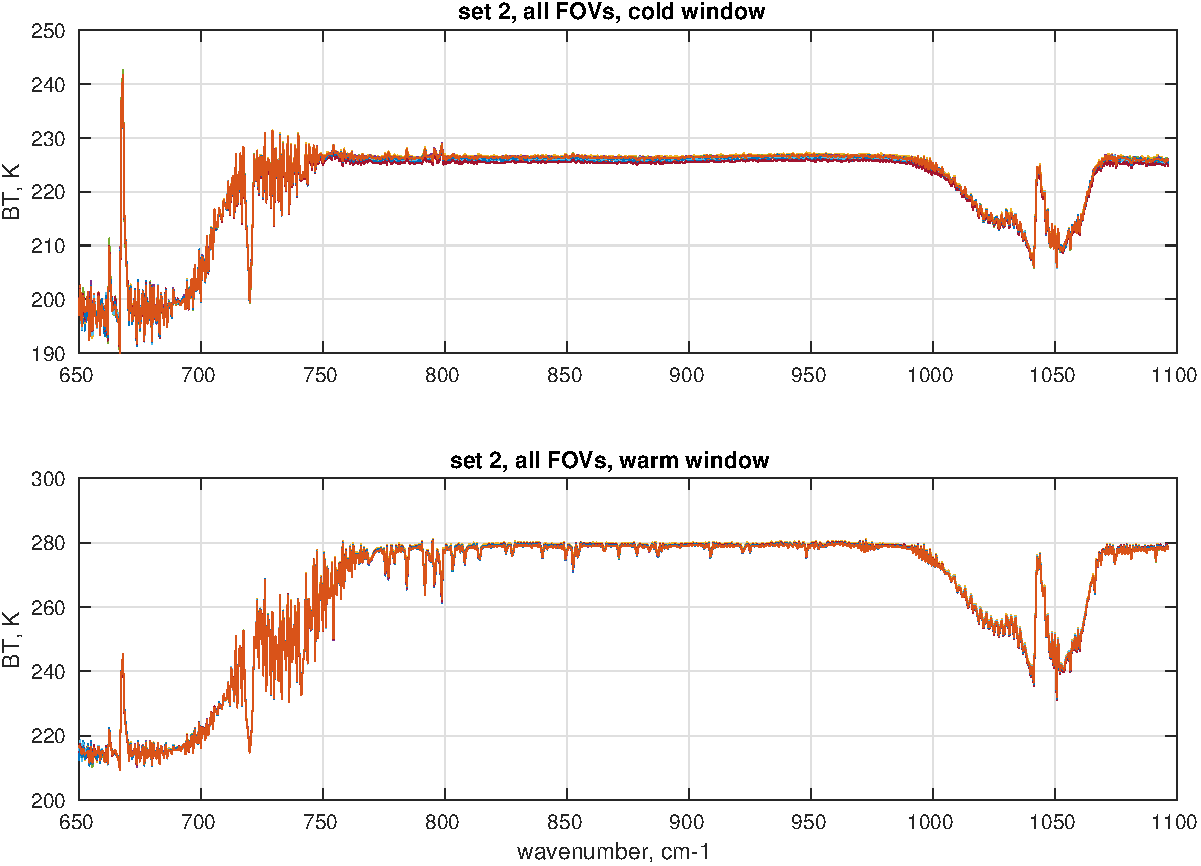
\includegraphics[scale=0.5]{figures/set2_all.pdf}
\end{center}
\end{frame}
%----------- slide --------------------------------------------------%
\begin{frame}
\frametitle{test set 3}
\begin{center}
  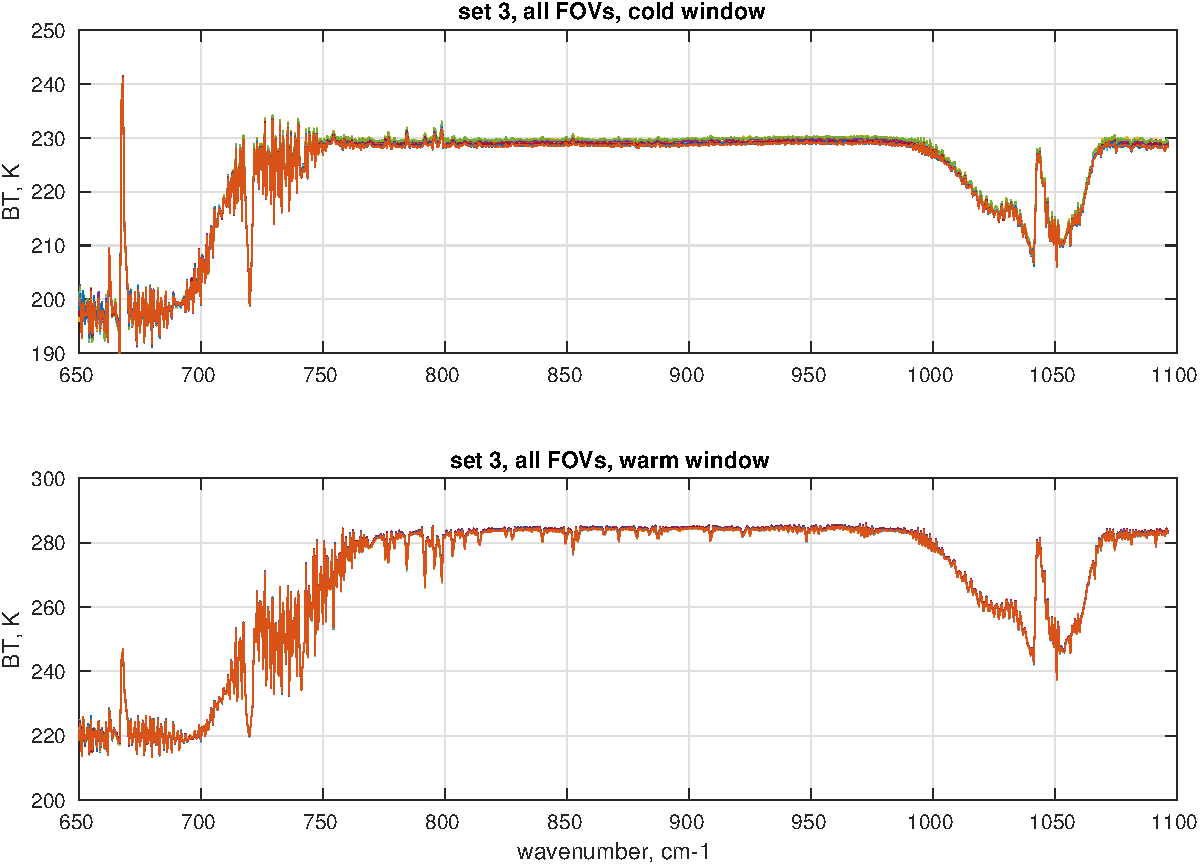
\includegraphics[scale=0.5]{figures/set3_all.pdf}
\end{center}
\end{frame}
%----------- slide --------------------------------------------------%
\begin{frame}
\frametitle{668 cm-1 zoom}
\begin{center}
  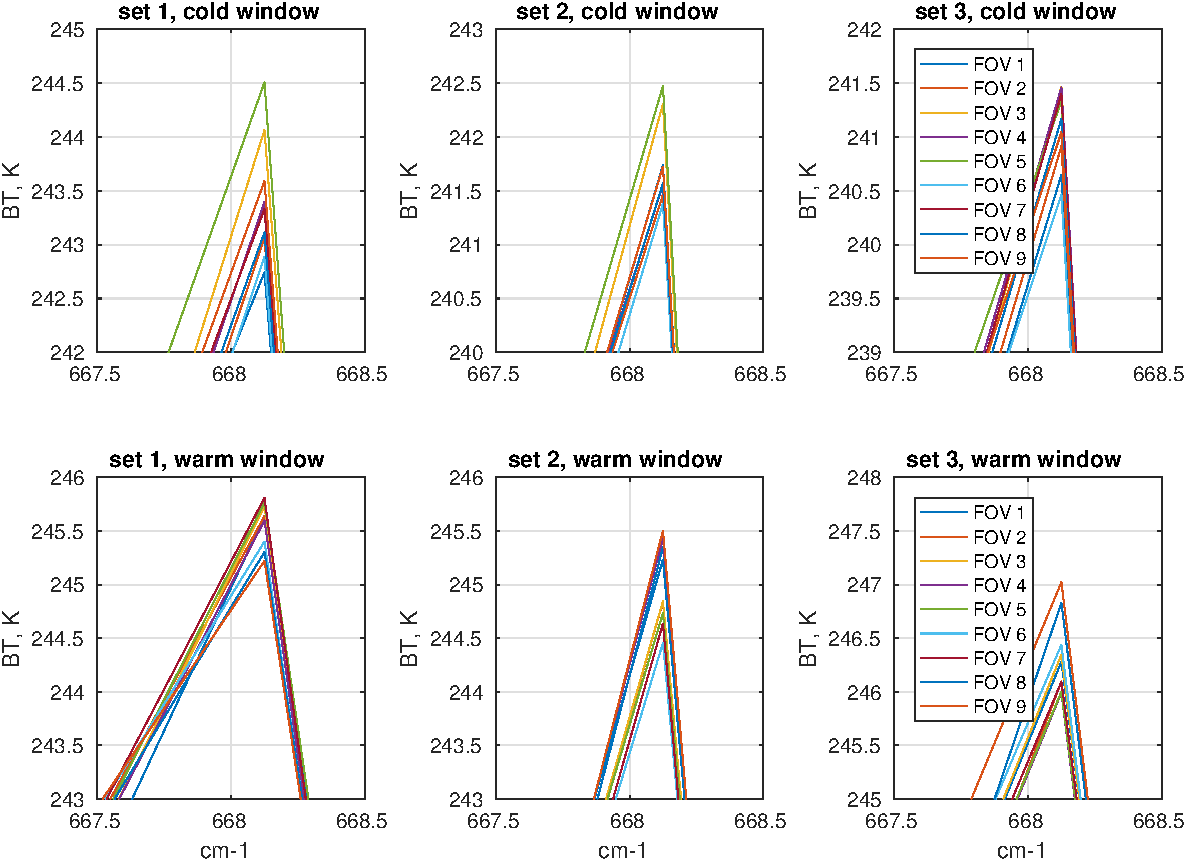
\includegraphics[scale=0.5]{figures/zoom_668.pdf}
\end{center}
\end{frame}

{ % begin nonlin definition scope
\newcommand {\rsp}   {r_{\mbox{\tiny sp}}}
\newcommand {\rins}  {r_{\mbox{\tiny in}}^{\mbox{\tiny s}}}
\newcommand {\rsps}  {r_{\mbox{\tiny sp}}^{\mbox{\tiny s}}}
\newcommand {\routs} {r_{\mbox{\tiny out}}^{\mbox{\tiny s}}}
\newcommand {\cm}    {c_{\mbox{\tiny m}}}
\newcommand {\cp}    {c_{\mbox{\tiny p}}}
\newcommand {\ca}    {c_{\mbox{\tiny a}}}
\newcommand {\vinst} {v_{\mbox{\tiny inst}}}
\newcommand {\vdc}   {v_{\mbox{\tiny dc}}}
\newcommand {\fn}    {f_{\mbox{\tiny N}}}
\newcommand {\fnm}   {f_{\mbox{\tiny NM}}}

%----------- slide --------------------------------------------------%
\begin{frame}
\frametitle{nonlinearity correction}

\begin{itemize}
 
 \item let $/$ be pointwise division, and
     \[\rins = \rin / \fn\]
     \[\rsps = \rsp / \fn\]

  \item the DC level is given by
    \[\vdc = \vinst + 
      \frac{2\cdot \sum_{i=1}^n|{\rins} - {\rsps}|} 
           {\cm \cdot \ca \cdot \cp \cdot d\cdot n}\]

  \item the corrected radiances (scaled by $\fn$) are
    \[\routs = \rins \cdot (1 + 2\cdot a_2 \cdot \vdc)\]

\end{itemize}

\end{frame}
%----------- slide --------------------------------------------------%
\begin{frame}
\frametitle{parameters}

\begin{itemize}
  \item $\rin$ is scene count spectra
  \item $\rsp$ is space-look count spectra
  \item $n$ is the number of decimated points
  \item $d$ is the decimation factor
  \item $\cm$ is modulation efficiency
  \item $\cp$ is PGA gain 
  \item $\ca$ is A/D gain
  \item $\vinst$ instrument contribution to DC level
  \item $\vdc$ is estimated DC level
  \item $\fn$ is the numeric filter at the sensor grid
  \item $a_2$ are the correction parameters
\end{itemize}

\end{frame}
} % end nonlin definition scope

%----------- slide --------------------------------------------------%
\begin{frame}[fragile]
\frametitle{DC Level Integral}

Values from the DC level integral\\
\begin{semiverbatim}\small
          set 1             set 2             set 3
FOV   cold     warm     cold     warm     cold     warm
 1   0.1190   0.3988   0.1157   0.3047   0.1231   0.3323
 2   0.1269   0.4202   0.1233   0.3233   0.1314   0.3476
 3   0.1188   0.3965   0.1173   0.3062   0.1251   0.3276
 4   0.1258   0.4171   0.1232   0.3192   0.1313   0.3476
 5   0.1353   0.4447   0.1312   0.3407   0.1409   0.3683
 6   0.1296   0.4250   0.1266   0.3291   0.1337   0.3552
 7   0.1343   0.4476   0.1292   0.3420   0.1387   0.3711
 8   0.1244   0.4188   0.1223   0.3196   0.1286   0.3458
 9   0.1155   0.3801   0.1117   0.2899   0.1170   0.3139
\end{semiverbatim}

\end{frame}
%----------- slide --------------------------------------------------%
\begin{frame}[fragile]
\frametitle{correction factor}

correction factor\\
\begin{semiverbatim}\small
          set 1             set 2             set 3
FOV   cold     warm     cold     warm     cold     warm
 1   1.0576   1.0684   1.0575   1.0648   1.0577   1.0659
 2   1.0443   1.0527   1.0442   1.0500   1.0445   1.0507
 3   1.0498   1.0588   1.0498   1.0558   1.0500   1.0565
 4   1.0677   1.0804   1.0676   1.0761   1.0679   1.0774
 5   1.0392   1.0475   1.0391   1.0447   1.0394   1.0455
 6   1.0523   1.0620   1.0522   1.0589   1.0525   1.0597
 7   1.0469   1.0560   1.0467   1.0530   1.0470   1.0538
 8   1.0529   1.0631   1.0528   1.0597   1.0530   1.0606
 9   1.0912   1.1073   1.0909   1.1018   1.0913   1.1033
\end{semiverbatim}

\end{frame}
%----------- slide --------------------------------------------------%
\begin{frame}
\frametitle{conclusions}

\begin{itemize}

  \item with the switch to extended res, we have seen a significant
    convergence in calibration algorithm performance 

  \item the {\noaa} ``SA-1 first'' algorithm does slightly better
    when compared with reference truth convolved with responsivity,
    while the {\ccast} ``ratio first'' algorithm does slightly
    better when compared with reference truth convolved with a flat
    passband

  \item this may be because responsivity cancels out more completely
    in the ratio-first method

  \item because reference truth convolved with a flat passband is a
    more conventional and non instrument-specific standard, the
    ccast algorithm, or some similar ratio-first method, may be
    preferable

\end{itemize}

\end{frame}
%----------- slide --------------------------------------------------%
\end{document}

